\newpage
\begin{center}
\section{Misura dell’effetto Zeeman normale}
\end{center}
\medskip
{\color{gray}\hrule}
\medskip
Inizialmente, inserita la lampada ai vapori di Cadmio tra le espansioni polari del magnete, si osserva la serie di anelli diffrattivi che, in assenza di campo magnetico applicato, corrisponde alla transizione atomica $3^1D_2 \rightarrow 2^1P_1$: essi sono il risultato dalla diseccitazione degli atomi di Cadmio che emettono fotoni con $\lambda=643.847$ nm. Per isolare questa transizione, dunque, si è inserito un filtro spettrale rosso nell'interferometro. 

In presenza di un campo magnetico esterno, i livelli energetici atomici si dividono secondo la relazione
\[
\Delta E = \mu_B \, \Delta m_l \, B ,
\]
dove $\mu_B$ è il magnetone di Bohr, $m_l$ è il numero quantico magnetico e $B$ l’intensità del campo applicato. A tale variazione di energia consegue una separazione delle lunghezze d’onda delle righe emesse, secondo 
\[
\Delta\!\left(\frac{1}{\lambda}\right) = \frac{\mu_B B}{hc}\,\Delta m_l .
\]
Si verifica quindi una separazione delle componenti spettrali, che risulta a sua volta proporzionale al campo magnetico applicato.

Nel caso dell’effetto Zeeman normale, per una transizione di dipolo, come quella del cadmio $3^1D_2 \rightarrow 2^1P_1$, sono permesse variazioni del numero quantico magnetico pari a
\[
\Delta m_l = 0, \pm 1 .
\]
Di conseguenza, una singola riga spettrale si sdoppia in tre componenti: una componente centrale $\pi$, corrispondente a $\Delta m_l = 0$, che risulta non spostata in quanto $\Delta E=0$, e due componenti $\sigma^{+}$ e $\sigma^{-}$, corrispondenti a $\Delta m_l = \pm 1$, spostate simmetricamente rispetto alla riga originaria. 

Osservando la radiazione lungo la direzione del campo magnetico (geometria longitudinale) si osservano solo le componenti $\sigma^{\pm}$, polarizzate circolarmente; osservando in direzione perpendicolare (geometria trasversale) si osservano invece tutte e tre le componenti: la componente $\pi$, polarizzata linearmente in direzione ortogonale al campo, e le due componenti $\sigma^{\pm}$, polarizzate linearmente sul piano ortogonale sia al campo, sia alle altre componenti.

\subsection{Effetto Zeeman in geometria longitudinale}

In configurazione longitudinale, ottenuta ruotando il supporto del magnete in modo che l'asse delle bobine sia in linea con la rotaia, l’asse ottico del sistema è dunque parallelo al campo magnetico. In questa geometria la componente $\pi$ non è osservabile, mentre le due componenti $\sigma^{+}$ e $\sigma^{-}$ risultano polarizzate circolarmente in versi opposti. Dopo aver verificato la separazione delle righe spettrali, dovuta all'applicazione di $B$, si posizionano la lamina $\lambda/4$ e il polarizzatore lineare,  tra le ultime due lenti convergenti, per selezionare alternativamente le due polarizzazioni circolari e osservare separatamente le due componenti.

La presa dati avviene in assenza degli elementi polarizzatori, acquisendo 9 diffrattogrammi al variare della corrente, quindi del campo magnetico, da 0A a circa 9A.\\
%Si prosegue posizionando la lamina e il filtro polarizzatore e riprendendo i diffrattogrammi avendo selezionato la componente $\sigma^{+}$ e poi la componente $\sigma^{-}$.
Dai diffrattogrammi, tramite un software di elaborazione immagini, si sono calcolate
le aree dei cerchi raffigurati, corrispondenti alle transizioni con
$\Delta m_l =\pm1$: ogni area è stata misurata 3 volte, per poter associare come
incertezza sulla media delle tre misure la loro semidispersione.
\begin{figure}[H]
    \centering
    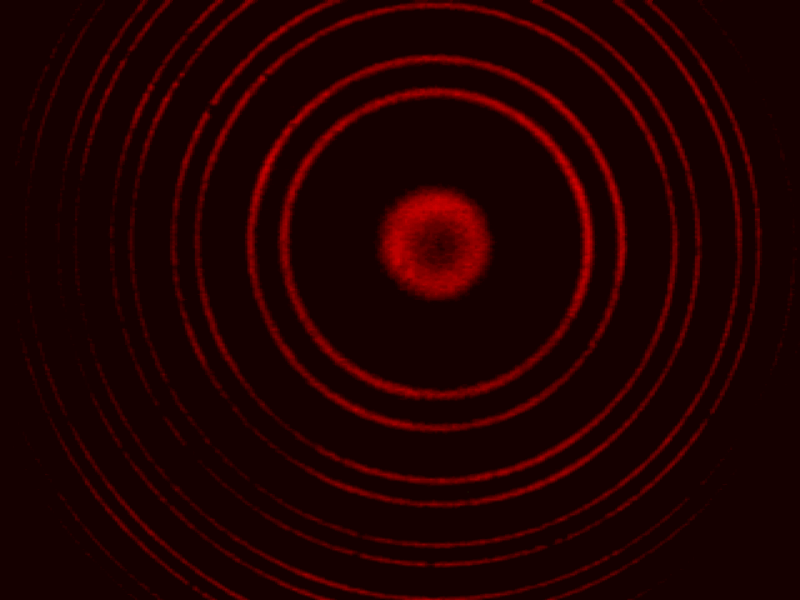
\includegraphics[width=.55\linewidth]{longit/1185.png}
    \caption{\footnotesize Diffrattogramma a $I=(6.1\pm0.3)$A in configurazione longitudinale: si noti
    lo splitting del pattern in due righe, che rappresentano le due transizioni con
    $\Delta m_l=\pm1$.}
\end{figure}
Per poter stimare il magnetone di Bohr, si devono ora definire due quantità:
\begin{itemize}
    \item $\delta_{a,b}$ differenza di area tra due massimi dello stesso ordine
	relativi a $\lambda_a,\lambda_b$ diverse, che non dipende dall'ordine di 
	massimo;
    \item $\Delta$ differenza di area tra due massimi di ordine consecutivo relativi
	alla stessa $\lambda$, che approssimativamente non dipende nè da $\lambda$, nè dall'ordine di massimo.
\end{itemize}
Il sistema ottico è stato tarato in modo da mostrare almeno 3 ordini di massimi di
interferenza, dunque per ogni diffrattogramma è stato possibile effettuare 3 stime di
$\delta_{a,b}$ e 4 di $\Delta$, di cui si è fatta una media pesata, ottenendo una coppia
di valori $\left(\langle\Delta\rangle,\langle\delta\rangle\right)$ per
diffrattogramma, cioè per valore di campo magnetico.\\
I valori di $\left(\langle\Delta\rangle,\langle\delta\rangle\right)$ al variare di $I$
per la configurazione longitudinale sono riportati in appendice \ref{sec:longit}.

Da questo set di dati sarà possibile estrarre una stima del magnetone di Bohr $\mu_B$ attraverso
i rapporti $\frac{\langle\delta\rangle}{\langle\Delta\rangle}$, anch'essi riportati in appendice
\ref{sec:longit}.
%INSERIRE GRAFICI E ANALISI DATI SPIEGATA, fino al calcolo sperimentale di $\frac{\langle \delta \rangle}{\langle \Delta \rangle}$
\subsection{Effetto Zeeman in geometria trasversale}

Si è poi messo il magnete in posizione trasversale, cioè in modo che l’asse ottico fosse perpendicolare al campo magnetico applicato. In questo caso, in presenza di campo magnetico, si osservano simultaneamente tre componenti: la componente centrale $\pi$, invariata in lunghezza d'onda, e le due componenti $\sigma^{\pm}$ simmetriche rispetto a $\pi$. La componente $\pi$ è polarizzata linearmente nella direzione del campo magnetico, mentre le componenti $\sigma^{\pm}$ risultano polarizzate linearmente sul piano ortogonale al campo magnetico.
Utilizzando un polarizzatore lineare si sono osservate separatamente le diverse componenti della luce in uscita dall'interferometro.

Anche in questa configurazione, la presa dati avviene in assenza del filtro polarizzatore, acquisendo 7 diffrattogrammi al variare della corrente da 0A a circa 9.5A.\\
%Si prosegue posizionando il filtro e riprendendo i diffrattogrammi prima avendo selezionato la componente $\sigma^{\pm}$ e poi la componente $\pi$.
Dalle immagini acquisite si sono poi calcolate le aree dei cerchi dei
diffrattogrammi, stimandole con media e semidispersione di 3 diverse misure.
\begin{figure}[H]
    \centering
    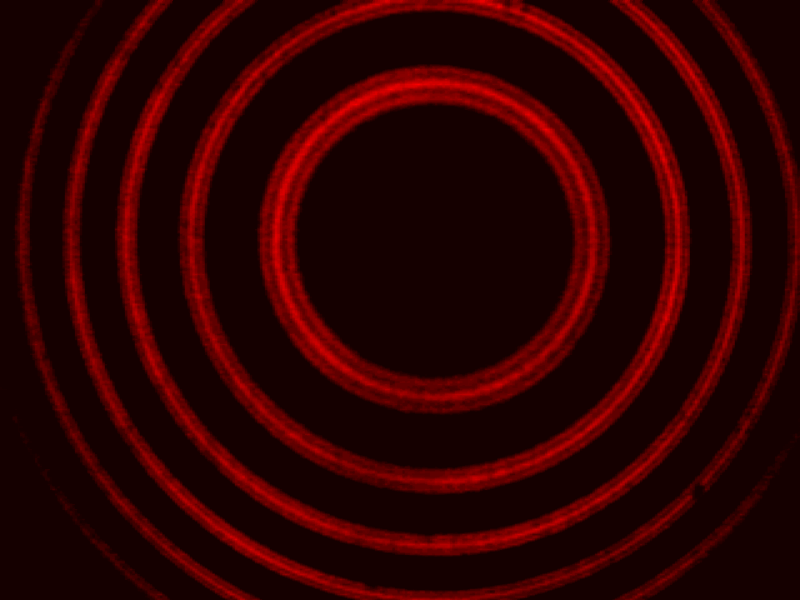
\includegraphics[width=.55\linewidth]{trasv/1191.png}
    \caption{\footnotesize Diffrattogramma a $I=(4.8\pm0.2)$A in configurazione longitudinale: si noti
    lo splitting del pattern in tre righe, che rappresentano le tre transizioni con
    $\Delta m_l=0,\pm1$. Questo diffrattogramma è stato scartato dall'analisi dati per la
    difficoltà di distinguere le diverse righe.}
\end{figure}
In questa configurazione si sono stimati i valori di $(\langle\Delta\rangle,\langle\delta\rangle)$
in modo diverso: si sono considerate separatamente la riga relativa alla transizione con
$\Delta m_l=+1$ (cioè quella esterna rispetto alla riga centrale) e quella alla transizione con
$\Delta m_l=-1$; per ciascuna transizione si sono stimati separatamente i valori di $\langle\Delta\rangle$ e 
$\langle\delta\rangle$ esattamente come si è fatto per la configurazione longitudinale.\\
I valori di $\left(\langle\Delta\rangle,\langle\delta\rangle\right)$ al variare di $I$ per entrambe le coppie di 
righe sono riportati in appendice \ref{sec:trasv}.\\
Da questi set di dati sarà possibile estrarre 2 stime del magnetone
di Bohr $\mu_B$ (una per coppia), attraverso i rapporti $\frac{\langle\delta\rangle}{\langle\Delta\rangle}$, anch'essi riportati in appendice
\ref{sec:trasv}.
%INSERIRE GRAFICI E ANALISI DATI SPIEGATA, fino al calcolo sperimentale di $\frac{\langle \delta \rangle}{\langle \Delta \rangle}$






